\documentclass[twocolumn]{jsarticle}
\usepackage{summary}
\usepackage[dvipdfmx]{graphicx}	%	図を取り込む		(推奨)
\usepackage{enumitem}
\usepackage{caption} % caption パッケージの追加
\captionsetup{
  format=hang, % キャプションをハングインデント(吊り込み)形式にする
	labelsep=space, % キャプションとラベルの間のスペースを空ける
}
\title{遅延聴覚フィードバックがもたらす影響の客観的な評価方法の検討と年齢による影響の変化の分析}
\author{山下\hspace{1zw}一樹}
\begin{document}
\maketitle

\section{はじめに}
\subsection{背景}
本節では,ディジタル補聴器の進化と課題について解説する.
ディジタル補聴器は,ディジタル信号処理を用いて従来のアナログ補聴器より高度な機能を実現しているが,
利用者からは十分な満足度が得られていないという問題が報告されている\cite{cf:Manzokudo}.
性能向上のためには精緻なディジタル信号処理と周波数帯域の細分化が必要だが,これは音声信号の長さを増加させ,
遅延時間の問題を引き起こす.ところで人は能動的な活動を行う際,活動とそれに伴う感覚フィードバックを対応付けることで
行動の調整を行っている.この中で,聴覚に関するフィードバックを聴覚フィードバックと呼ぶ\cite{cf:DAF}.
一般に聴覚フィードバックの遅延時間が10[ms]を超えると,発話や身体運動に影響を与えることが知られている\cite{cf:DelayTime-ninnchi}.
特に,ディジタル補聴器における遅延時間もこの遅延時間に該当し,
この遅延時間を短縮しつつ高度な処理を実現することが困難である.
しかし,高齢者は遅延時間が10[ms]を超えても違和感を覚えにくいことから,
この知見を利用して遅延時間を増大させることで,より高度なディジタル信号処理を実装することが期待される.
\subsection{目的}
本研究では,若年者と高齢者の聴覚フィードバックの遅延時間の許容量の差を調査し,
聴覚フィードバックによる違和感を客観的に評価するため,聴覚フィードバックの
遅延が身体運動に与える影響を検討する.
遅延聴覚フィードバックの影響を幅広い年代で比較することを想定して,簡易なボタン押し課題を採用する.
この課題では,メトロノームの合図音に合わせてボタンを押す動作を行い,遅延の影響を分析する.
先行研究\cite{cf:kayama}では,遅延聴覚フィードバックが発話に与える影響について検討されたが,
この研究は主観評価に基づくもので,個人差が顕著であるという問題があった.
そこで,本研究では,遅延聴覚フィードバックによる影響を客観的に評価するため,
先行研究\cite{cf:shigematu}で著者らによって行われた調査のシステムについて改良を行う.
遅延による影響の大きさを探るため,ボタン押し課題の最適な条件を検討し,若年者と高齢者を対象に影響の調査を行う.
本研究は,聴覚フィードバックの遅延が身体運動に与える影響と年齢差の関係を明らかにし,
高齢者向け補聴器の設計において重要な示唆を提供することが期待される.

% \section{主観評価におけるアプリケーション開発}
先行研究\cite{cf:kayama}で著者らは,遅延聴覚フィードバックが発話に与える影響について,主観評価実験を行った.
主観評価実験とは,耳介付近に伝達された音に一定の遅延を発生させて外耳道に出力する装置を装着した被験者が,
発話時の違和感を主観的に評価するという内容の調査である.
本節では,開発したアプリケーションの概要を説明し,これを主観評価実験で利用することを想定する.
このアプリケーションにより,データ入力ミスのリスクが減少し,
実験者の負担が軽減されることで,より効率的に多くの実験を実施し,結果を分析することが可能になる.
アプリケーションの外観を図\ref{fig:2_userInterface}に示す.
\begin{figure}[tbp]
  \centering
  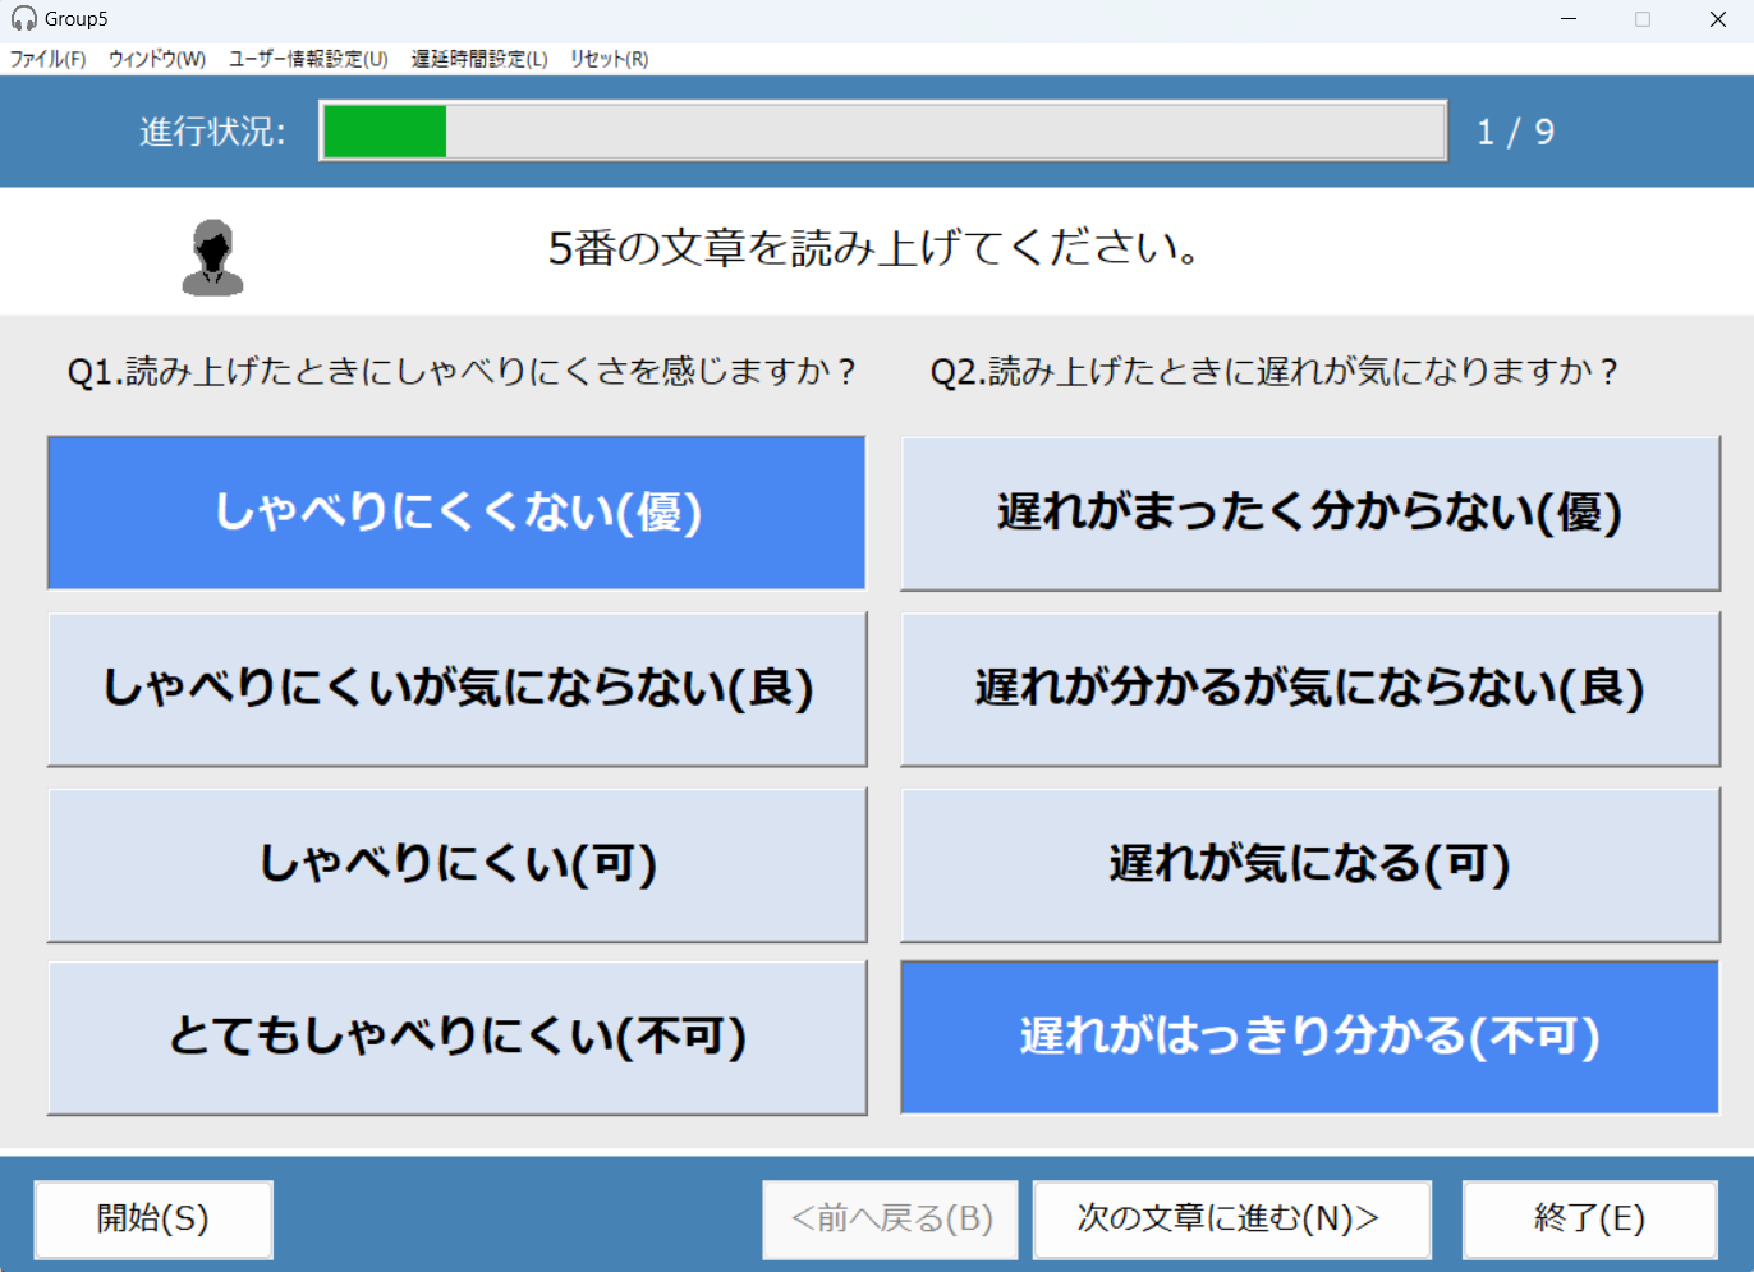
\includegraphics[scale=0.22]{figures/Syukann/app_2.pdf}
  \caption{調査中の画面}
  \label{fig:2_userInterface}
\end{figure}
\section{ボタン押し課題のシステム}
\subsection{ボタン押し課題}
本研究で行う客観評価による調査では,被験者が行う課題にボタン押し課題を採用する.
この調査で採用するボタン押し課題は,コントローラのボタンを押下するとクリック音が再生されるシステムを使用し,
このクリック音に遅延を発生させて被験者に聞かせながら,被験者が一定の時間間隔でボタンを押下する課題を行うというものである.
このボタン押し課題を用いて,遅延聴覚フィードバックが身体運動に与える影響を様々な年代の被験者について調査することが可能になると考えられる.
被験者がボタンを押す時間間隔を記録し,被験者がボタンを押したときに出力されるクリック音に遅延を加えることでそのばらつきがどのように変化するかを調査する.
この方法により,遅延聴覚フィードバックが身体運動に与える影響を客観的に評価することが可能になると考えられる.
また,馴化による効果を考慮するため,ボタンの押下回数が4の倍数に到達したときのみ,聴覚フィードバックの遅延を発生させた.
この課題を行うために,被験者が使用するシステムの構成を図\ref{fig:button-click-system}に示す.
\begin{figure}[tb]
  \centering
  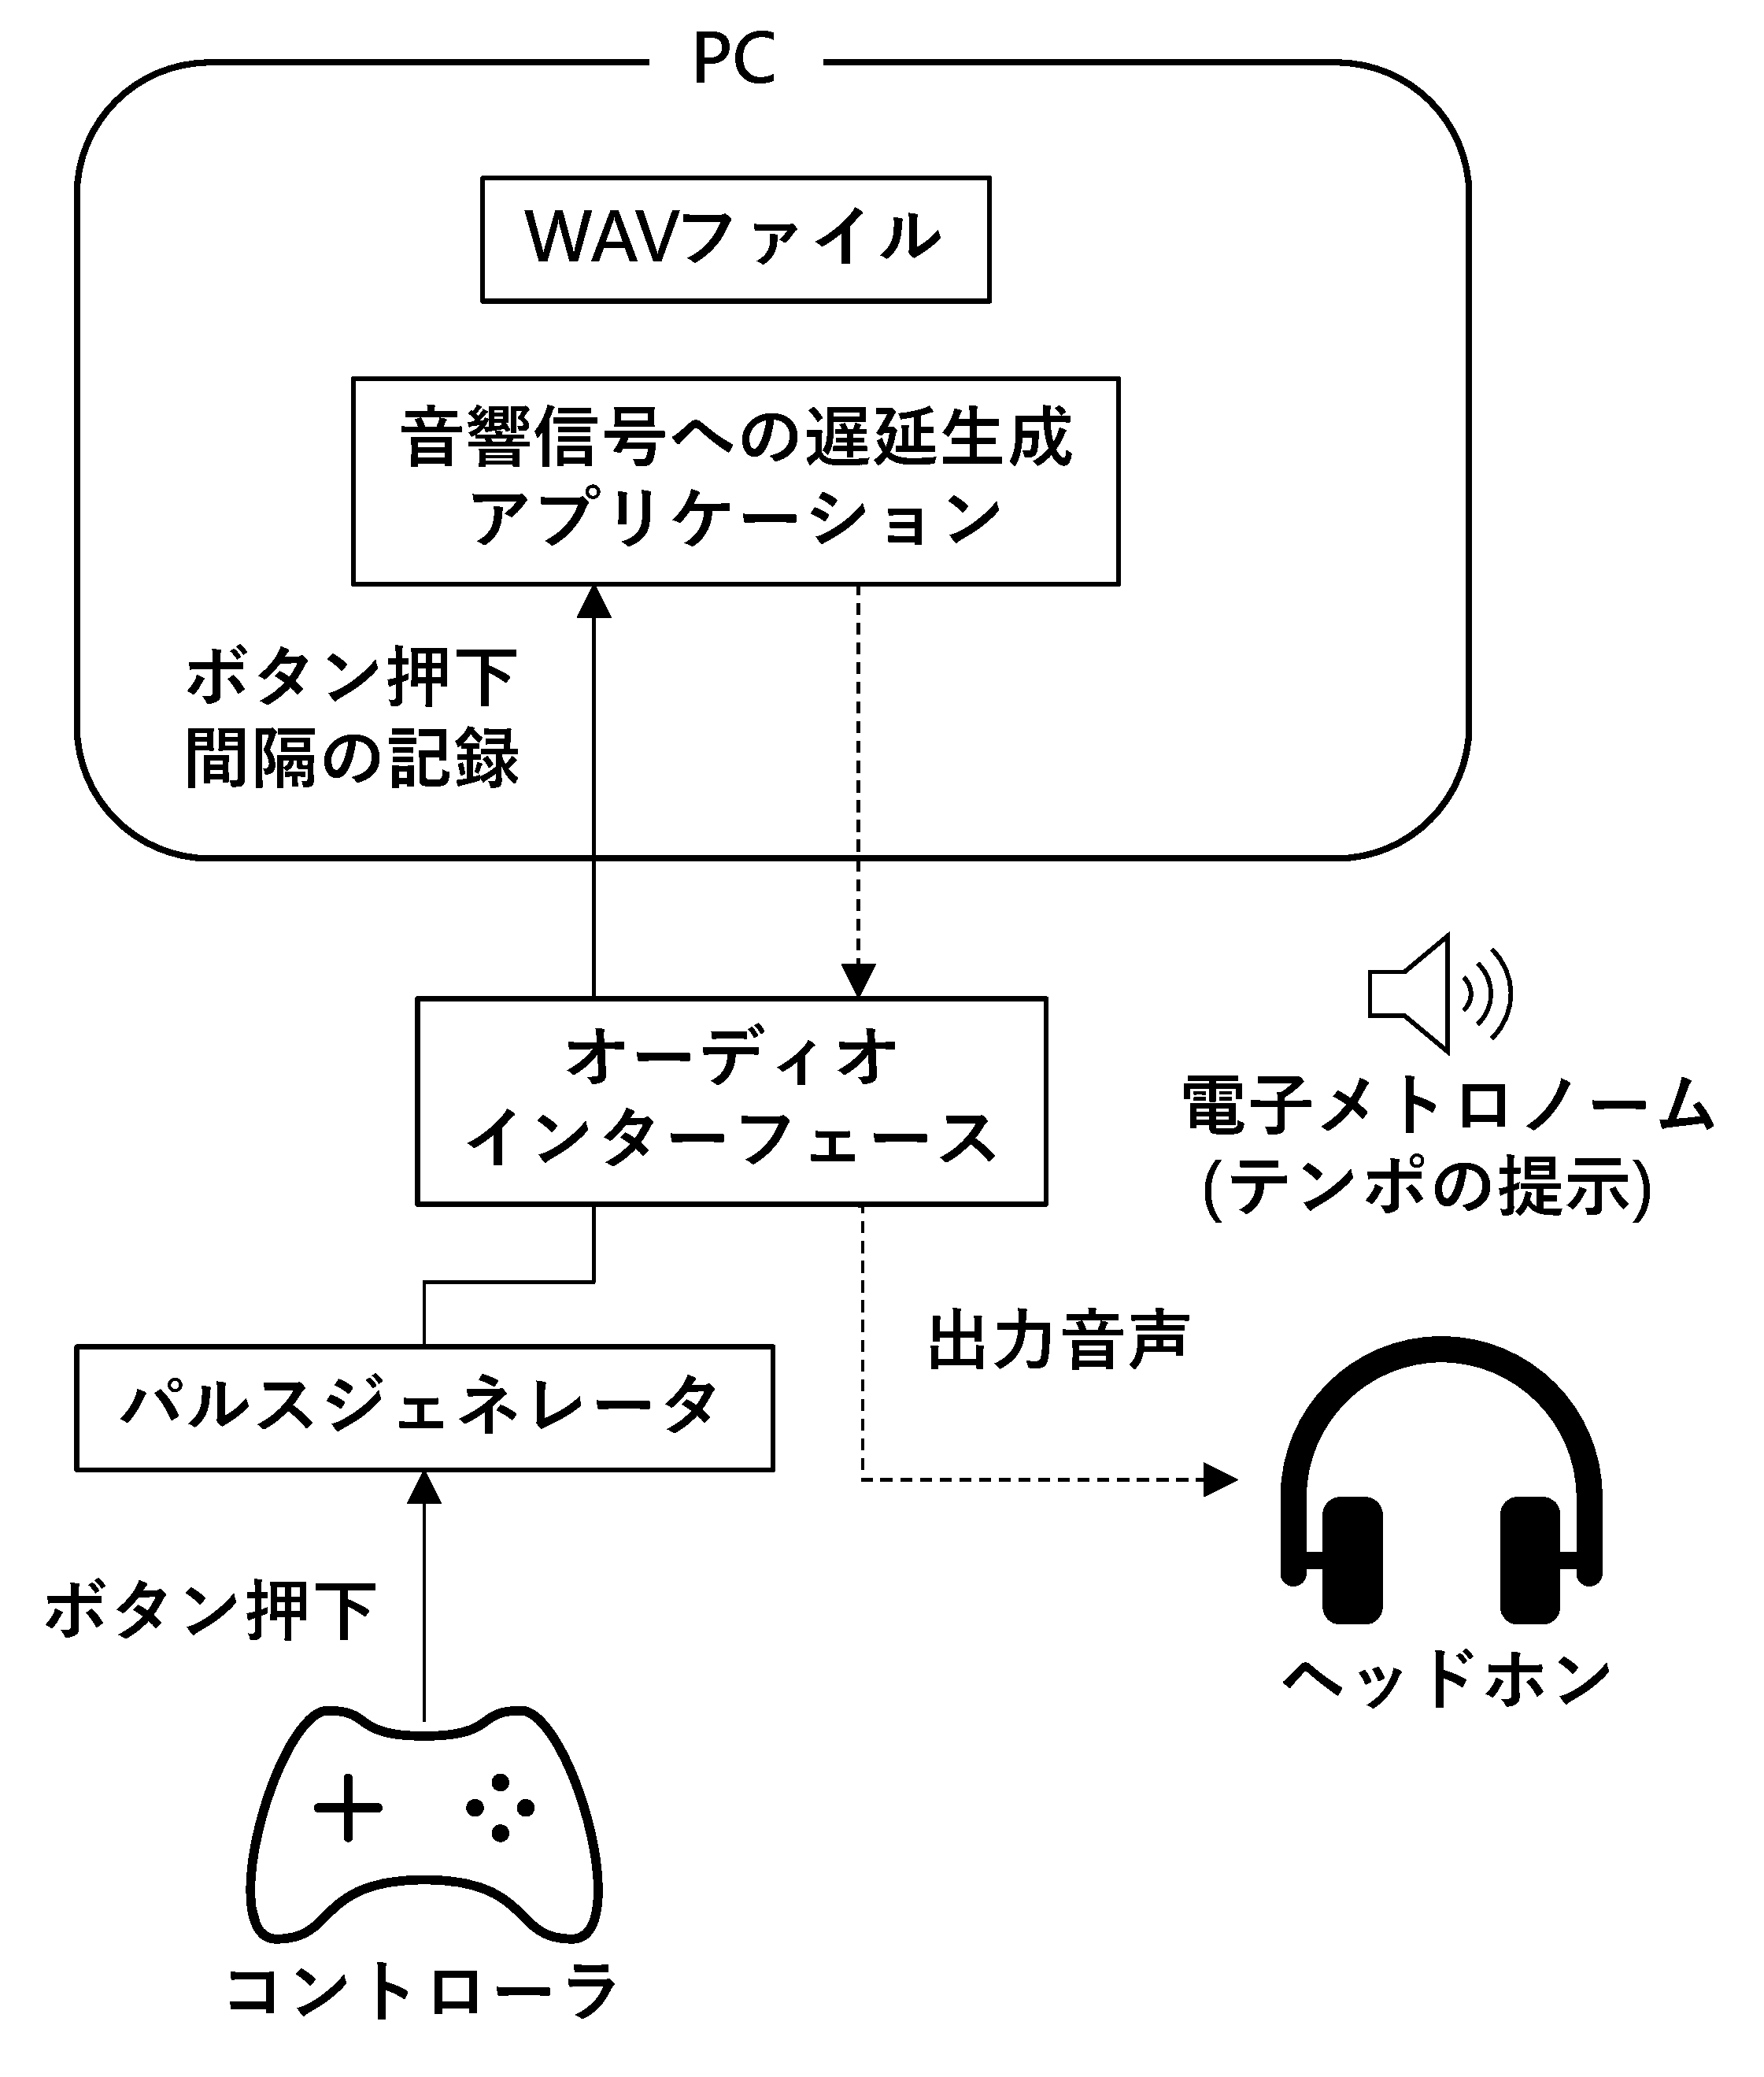
\includegraphics[scale=0.15]{figures/system_button_click.pdf}
  \caption{調査システムの構成}
  \label{fig:button-click-system}
\end{figure}
\subsection{音響信号への遅延生成アプリケーション}
本研究で使用する音響信号への遅延生成アプリケーションは,オーディオドライバにASIO(Audio Stream Input Output)を使用し,
図\ref{fig:button-click-system}に示すように,コントローラのボタンが押下されてから任意の遅延時間後にボタン押下の合図音であるクリック音のWAVファイルがヘッドホンから出力される仕組みを有している.
このアプリケーションの表示例を図\ref{fig:app_kyakkann}に示す.
\begin{figure}[tbp]
  \centering
  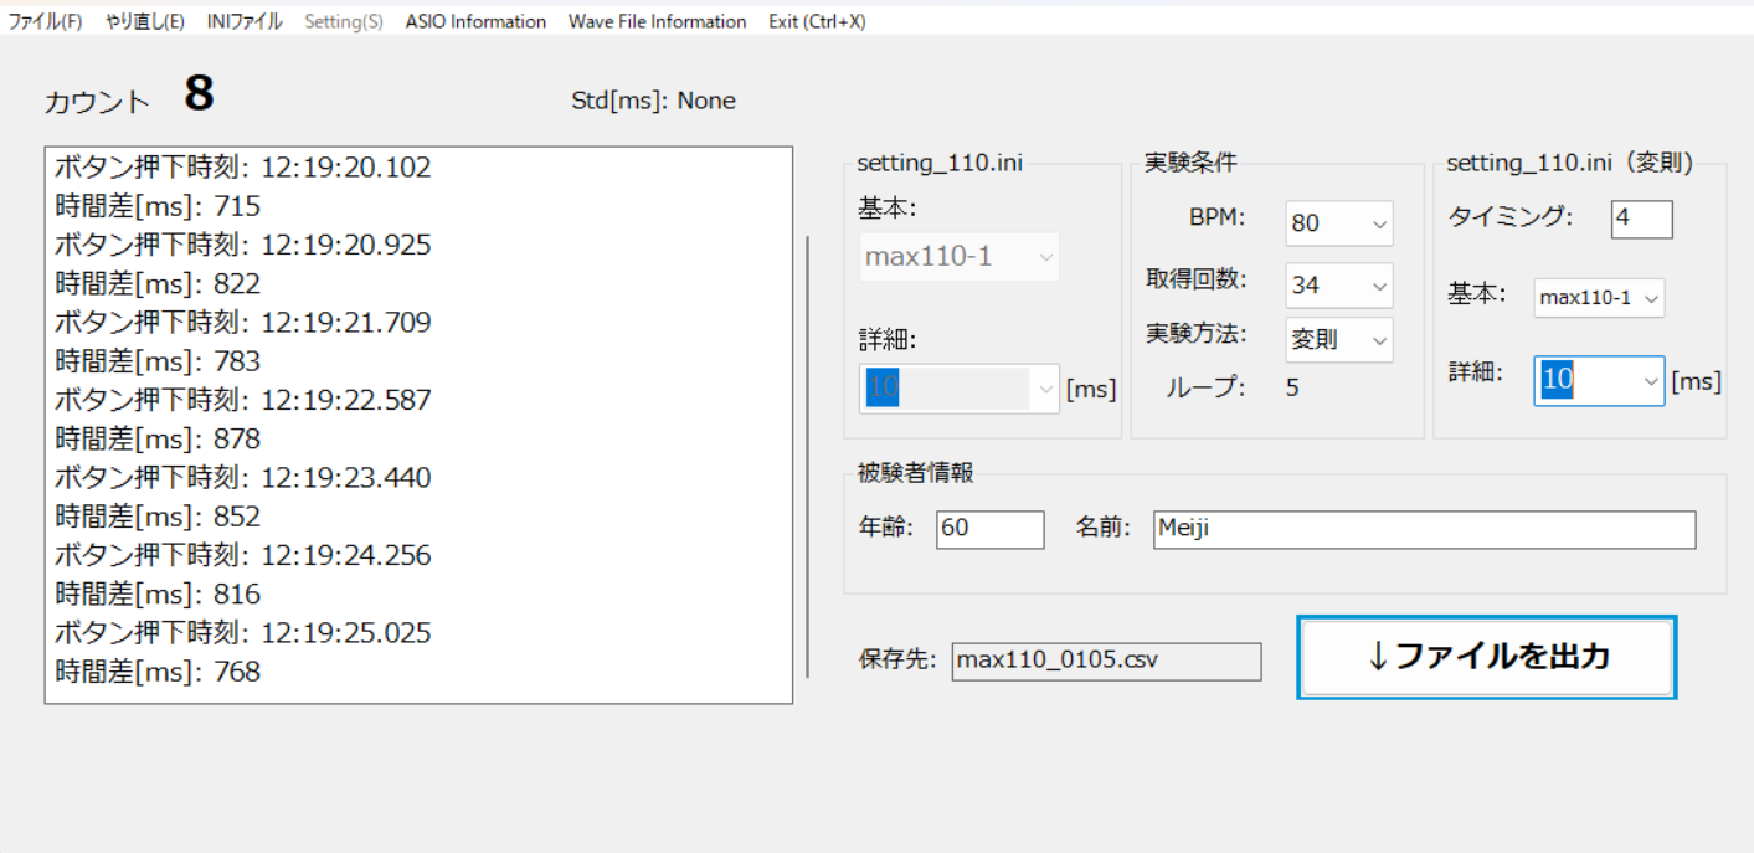
\includegraphics[scale=0.22]{figures/Apprication/App_kyakkann.pdf}
  \caption{音響信号への遅延生成アプリケーションの画面の表示例}
  \label{fig:app_kyakkann}
\end{figure}
本アプリケーションは,実験者が画面上のコンボボックスで指定した時間だけ遅延させる機能や被験者がボタンを押下する時間間隔を記録する機能を持つ.
本研究では,このアプリケーションを使用して,遅延聴覚フィードバックの身体運動への影響を調査した.
\section{評価方法}
遅延聴覚フィードバックが身体運動に与える影響の評価は,被験者が行うボタン押下の時間間隔の分散と
遅延が4の倍数に到達したときのみ発生する状況を考慮して,4の倍数に到達する直前のボタンの押下間隔と
直後のボタン押下間隔のデータの差の二乗平均(Mean Squared Error, MSE)および誤差の中央値(Median Squared Error, MedSE)を用いて行う.
この評価方法は,遅延聴覚フィードバックが身体運動に影響を与えている場合,遅延が発生する直前のボタン押下間隔と
直後のボタン押下間隔の差が大きくなることを想定している.
% 以下にこれらの評価指標の定義を示す.
% \begin{equation}
%   s^2_a = \frac{1}{l-1} \sum_{i=k}^{k+l-1} (x_i - \bar{x}_{kl})^2
% \end{equation}
% \begin{equation}
%   s^2_b = \frac{1}{l} \sum_{i=k}^{k+l-1} (x_i - M_{kl})^2
% \end{equation}
% \begin{equation}
%   s^2_c = \frac{1}{l} \sum_{i=k}^{k+l-1} (x_i - T)^2
% \end{equation}
% \begin{equation}
%   f(n) = \left\lfloor \frac{n-t-1}{t} \right\rfloor + 1
% \end{equation}
% \begin{equation}
%   s(n) = \left\lfloor \frac{n-t-2}{t-1} \right\rfloor
% \end{equation}
\section{遅延聴覚フィードバックが身体運動に与える影響の調査}
\subsection{調査方法}
聴覚フィードバックの遅延時間を多様に設定し,一定間隔でのボタン押下時の時間間隔のばらつきを調査した.
改良したシステムでは,ボタンの押下回数が4の倍数に達するごとに遅延を発生させた.
遅延時間は被験者には非公開として,発生させる遅延時間の順番はランダムとした.
設定した遅延時間は,実験Aでは20ms間隔で10-110ms,実験Bでは5ms間隔で10-40msとした.
実験Aの被験者は若年者(21-25歳)38名と高齢者(60-82歳)41名,実験Bの被験者は若年者(20-25歳)34名と高齢者(60-64歳)40名である.
ボタン押下の間隔は毎分80回,ボタン押下回数は34回とした.
遅延時間の提示順序は,最初に10[ms]を提示し,次に10[ms]以外の中からランダムに選択し提示する.
その後,残る遅延時間に10[ms]を加えたものをランダムに提示する.
得られた結果は,遅延時間に応じて各被験者の観測値の四分位範囲(IQR)と第一・第三四分位数を算出し,
外れ値を除外するために第一四分位数-1.5×IQR以下と第三四分位数+1.5×IQR以上の値を排除して,
4章で述べた評価方法により分析した.
\subsection{調査結果}
図\ref{fig:Normalized-Var_40ms_SaSbSc}および図\ref{fig:Normalized_40ms_MSE_MedSE}に示した
10[ms]から40[ms]の短い遅延時間帯における観察結果から,若年者の反応は遅延時間の増加に伴い緩やかに増加する傾向にあるが,
高齢者の反応には一貫した関係が認められないことが示された.このことは,若年者が遅延に対して敏感であり,一方で高齢者が遅延時間に対してある程度の
許容度を持っていることを示唆している.
一方,図\ref{fig:Normalized-Var_110ms_SaSbSc}および図\ref{fig:Normalized_110ms_MSE_MedSE}より,
遅延時間を10[ms]から110[ms]に拡大した場合,特に90[ms]を超える長い遅延時間帯における高齢者の反応に大幅な増加が観察され,高齢者が遅延時間の
増加に対して比較的鈍感であるものの,90[ms]を超えるとタスクの一貫性を保つことが困難になることが示された.
若年者も長い遅延時間において,反応の増加を示したが,この増加は高齢者ほど急激ではなかった.
これらの結果は,遅延時間が増加するにつれて若年者と高齢者の反応の差異が顕著になることを示し,
若年者は短い遅延時間帯でも遅延を感じやすく,高齢者は長い遅延時間において特に顕著な反応を示したことを明らかにする.
さらに,遅延時間に対する年齢別の感受性の違いは,遅延聴覚フィードバックにおける効果を最大化するための異なるアプローチの
重要性を協調している.
\begin{figure}[tbp]
  \centering
  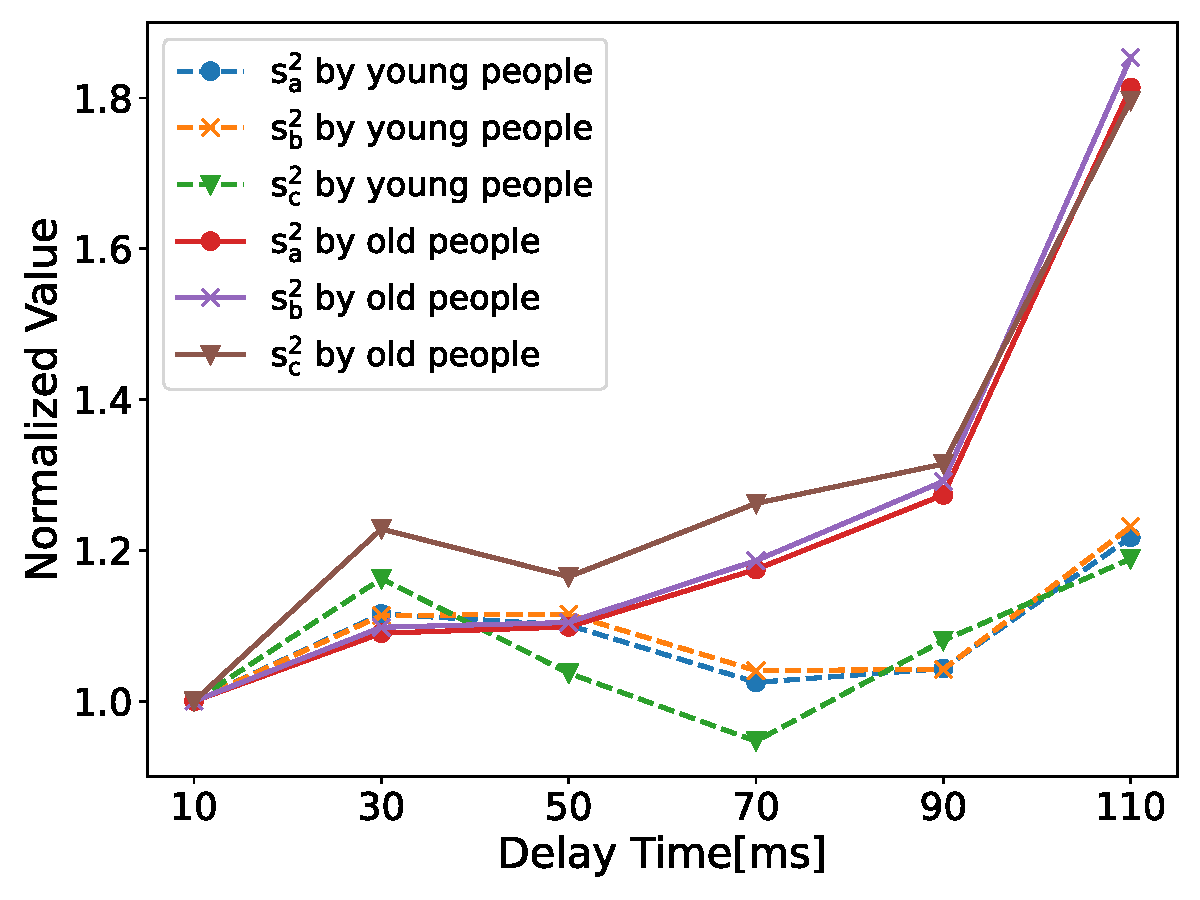
\includegraphics[scale=0.3]{figures/Honbann/Comparison_young_old/110_var_normalized.pdf}
  \caption{実験Aにおける若年者と高齢者の正規化後の評価値の比較}
  \label{fig:Normalized-Var_110ms_SaSbSc}
\end{figure}
\begin{figure}[tbp]
  \centering
  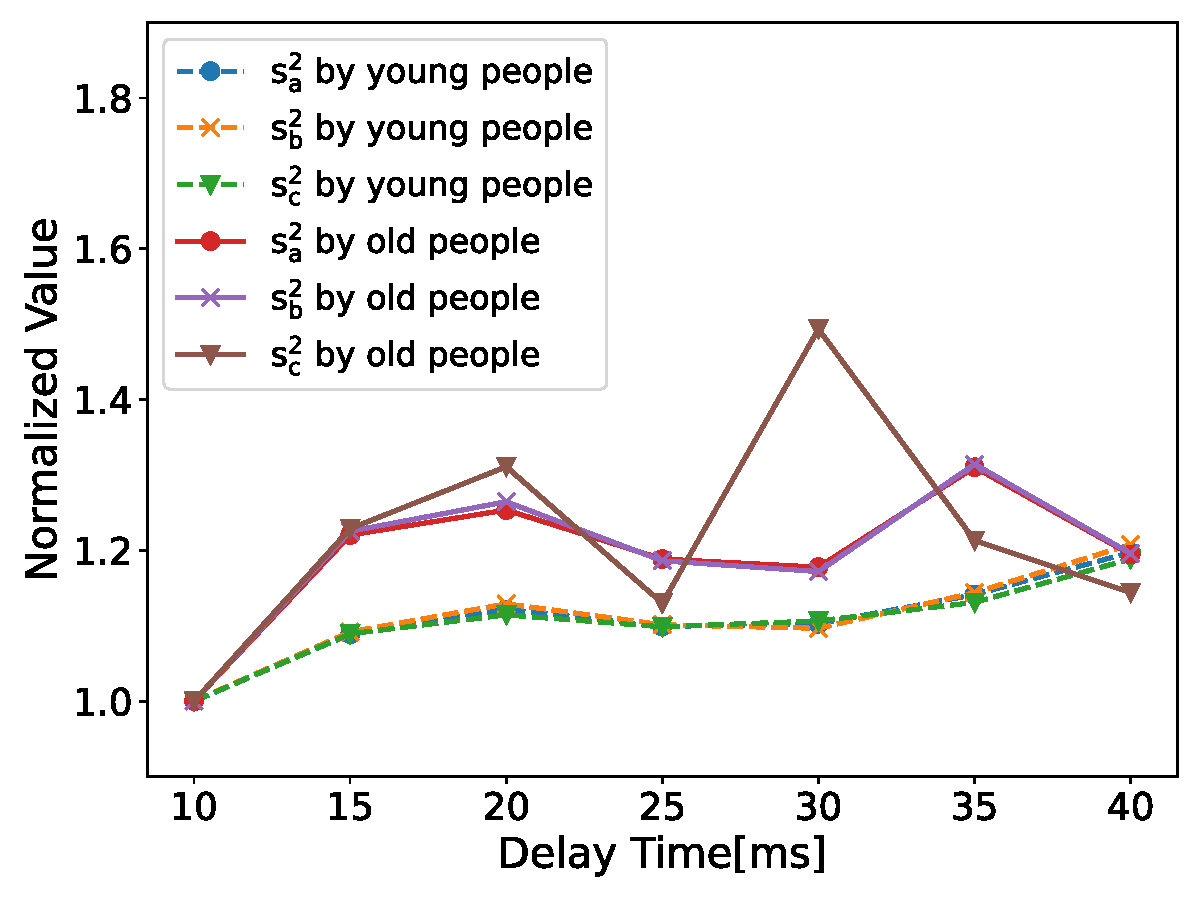
\includegraphics[scale=0.3]{figures/Honbann/Comparison_young_old/40_var_normalized.pdf}
  \caption{実験Bにおける若年者と高齢者の正規化後の評価値の比較}
  \label{fig:Normalized-Var_40ms_SaSbSc}
\end{figure}
\begin{figure}[tbp]
  \centering
  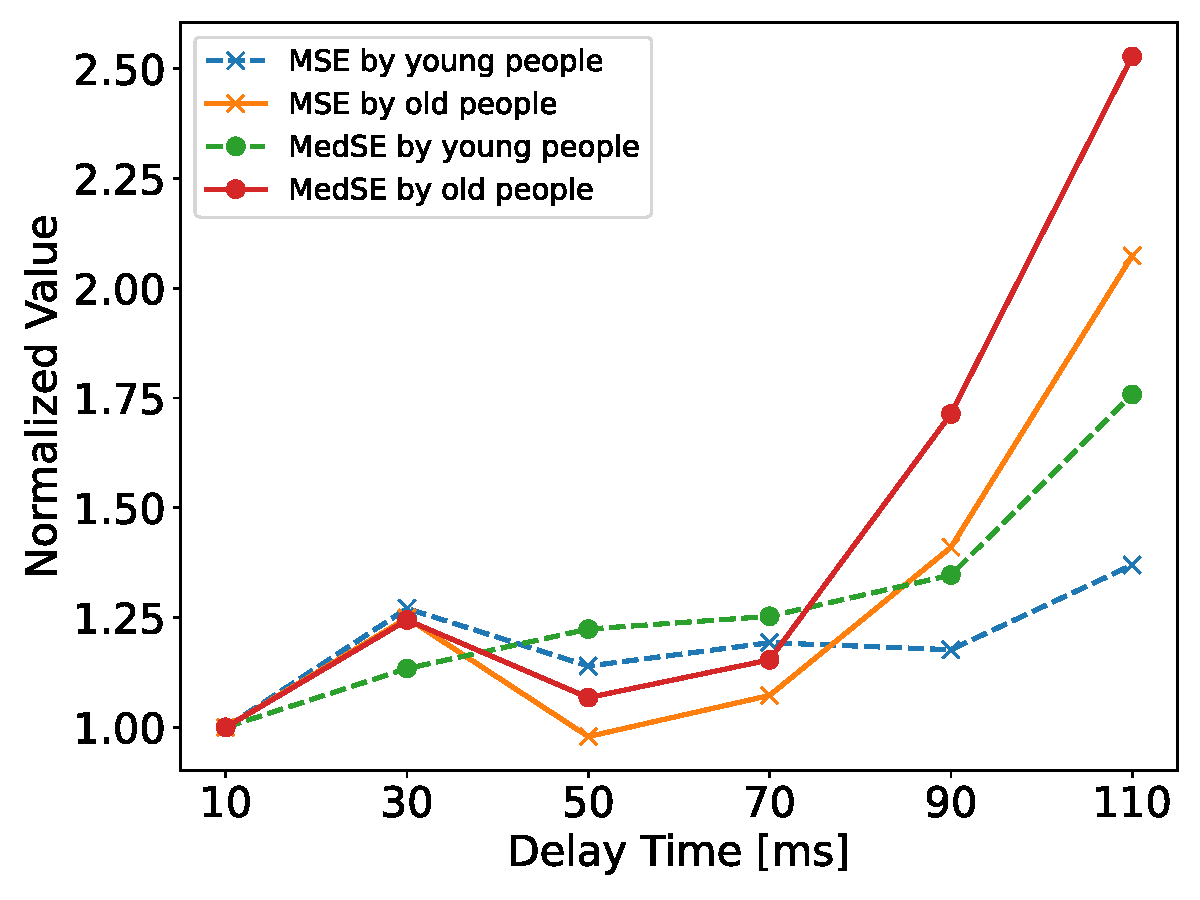
\includegraphics[scale=0.3]{figures/Honbann/Comparison_young_old/110_MSE-MedSE_normalized.pdf}
  \caption{実験Aにおける若年者と高齢者の正規化後のMSEとMedSEの比較}
  \label{fig:Normalized_110ms_MSE_MedSE}
\end{figure}
\begin{figure}[tbp]
  \centering
  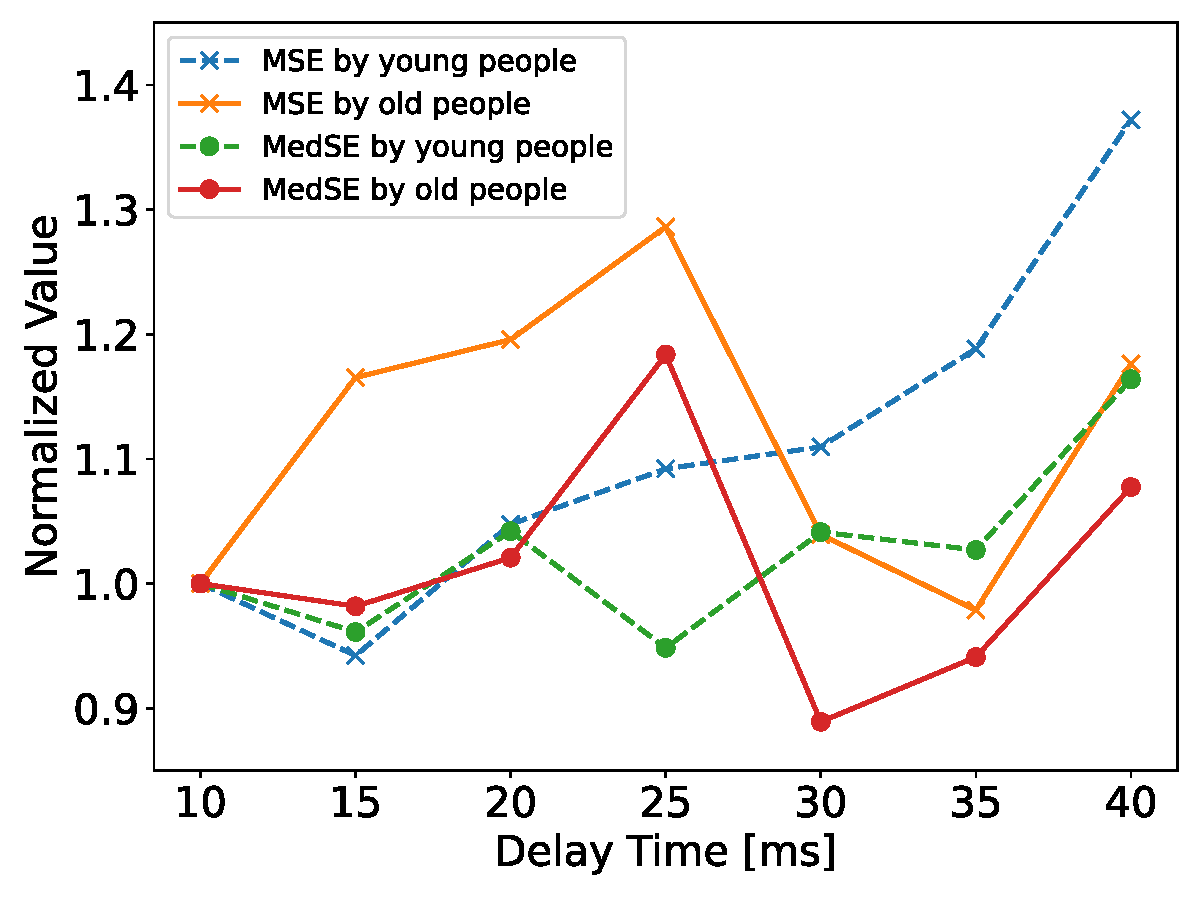
\includegraphics[scale=0.3]{figures/Honbann/Comparison_young_old/40_MSE-MedSE_normalized.pdf}
  \caption{実験Bにおける若年者と高齢者の正規化後のMSEとMedSEの比較}
  \label{fig:Normalized_40ms_MSE_MedSE}
\end{figure}
\section{結論}
\subsection{まとめ}
本研究では,文献\cite{cf:shigematu}の調査システムを改良し,改良後の調査システムを利用したボタン押し課題を用いて,
遅延聴覚フィードバックが身体運動にもたらす影響の客観的な評価方法を検討し,若年者と高齢者を対象に調査した.
遅延聴覚フィードバックの影響を観察するため,特定の条件下でボタン押し課題を行い,
その結果を分析した.若年者と高齢者を対象にした調査から,
聴覚フィードバックの遅延時間に対する感受性において年齢による違いがあることが明らかになった.
若年者は遅延時間に対して敏感である一方で,高齢者は遅延時間に対して一定の許容度を持っている可能性が示唆された.
\subsection{今後の課題}
今後は,高齢者と若年者の運動能力の差異を考慮し,遅延聴覚フィードバックの影響を公平に評価するために,
運動能力に応じた課題の検討が必要である.
また,遅延聴覚フィードバックが発話に及ぼす影響の客観的な評価方法の検討および本研究で得られたデータとの比較も必要である.
これらは,補聴器の設計に役立つ知見を提供することが期待される.


\begin{thebibliography}{99}
	\bibitem{cf:Manzokudo}西山崇経,新田清一,鈴木大介,岡崎宏,坂本耕二,中村伸太郎,上野恵,小川郁,``補聴器装用者の満足度に関わる要因の検討'' Audiology Japan, 57巻,3号,pp.189-194, Jun.2014.
	\bibitem{cf:DAF}河原英紀,``聴覚フィードバックの発話への影響:ヒトは自分の話声を聞いているのか?'' 日本音響学会誌, 59巻, 11号, pp.670-675, Nov.2003.
	\bibitem{cf:DelayTime-ninnchi}硲田猛真,中村陽裕,福本儀智,長谷川賢作,北野博也,``ディレイタイムの認知閾値'' Ausiology Japan, 46巻, 5号, pp.465-467, Sep.2007.
	\bibitem{cf:shigematu}重松颯人,丹治寛樹,村上隆啓,松本直樹,``遅延聴覚フィードバックが身体運動に与える影響の客観的な評価方法の検討'' 日本音響学会聴覚研究会資料, pp.499-504, Nov.2019.
	\bibitem{cf:kayama}香山実結花,山下一樹,丹治寛樹,村上隆啓,``若年者と高齢者の聴覚フィードバックにおける遅延時間の許容量の統計的分析による比較'' 2022年度電子情報通信学会東京支部学生会研究発表会, pp.113, Mar.2023.
\end{thebibliography}

\begin{thepublished}{99}
	\bibitem{pub:a}山下一樹,安田和生,丹治寛樹,村上隆啓``,\<'' 2023年度電子情報通信学会東京支部学生会,Mar.2024.
\end{thepublished}
\end{document}
